\makeatother
%	\author{Mitesh M. Khapra}
	\title{Module 5}
	\subtitle{Faster, Higher, Stronger}
		\author{}
		\institute{}
	\date{}
%\institute{Department of Computer Science and Engineering\\ Indian Institute of Technology Madras}
%\titlegraphic{\includegraphics[height=1cm,width=2cm]{images/iitm_logo.png}}
%\titlegraphicii{\includegraphics[height=1cm,width=2cm]{logo2}}

\begin{frame}
	\myheading{Chapter 5: Faster, higher, stronger}
\end{frame}

\begin{frame}
\begin{minipage}[t][0.6\textheight][t]{\textwidth}
\begin{columns}


\column{0.5\textwidth}
\begin{overlayarea}{\textwidth}{\textheight}
\justify
\only<1->{\myheading{Better Optimization Methods} Faster convergence, better accuracies}
\end{overlayarea}
\column{0.5\textwidth}
\begin{overlayarea}{\textwidth}{\textheight}
\begin{figure}
\centering
\only<1->{\includegraphics[scale=0.3]{"images/sgd_quiver84"}}
\end{figure}
\end{overlayarea}

\end{columns}
\end{minipage}

\begin{minipage}[t][0.5\textheight][t]{\textwidth}
\begin{overlayarea}{\textwidth}{\textheight}
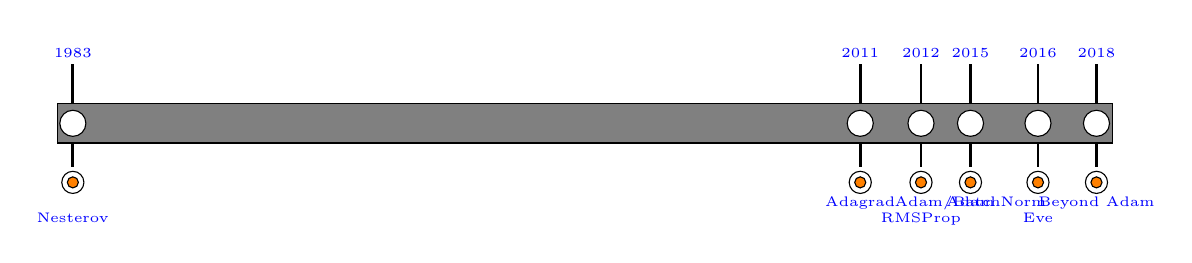
\begin{tikzpicture}[datemarker/.style={circle, draw=black,fill=white},textlabel/.style={anchor=center,text height=1.7ex,text depth=.25ex}]
\tikzset{every node/.style={font=\tiny, color=blue}}\draw[fill=gray](-0.2,0) rectangle (13.2,0.5) node[white, below]{};
\onslide<1->{\node at (0.0, 0.25) [datemarker] {};}
\onslide<1->{\draw [line width=1pt] (0.0, 0.5) to (0.0, 1.0);}
\onslide<1->{\draw (0.0, 1.2) node [textlabel]{1983};}
\onslide<1->{\draw [fill=orange](0.0, -0.5) circle (2pt){};}
\onslide<1->{\draw(0.0, -0.5) circle (4pt){};}
\onslide<1->{\draw [line width=1pt] (0.0, 0) to (0.0, -0.3);}
\onslide<1->{\draw (0.0,-0.9) node [textlabel] {Nesterov};}

\onslide<2->{\node at (10.0, 0.25) [datemarker] {};}
\onslide<2->{\draw [line width=1pt] (10.0, 0.5) to (10.0, 1.0);}
\onslide<2->{\draw (10.0, 1.2) node [textlabel]{2011};}
\onslide<2->{\draw [fill=orange](10.0, -0.5) circle (2pt){};}
\onslide<2->{\draw(10.0, -0.5) circle (4pt){};}
\onslide<2->{\draw [line width=1pt] (10.0, 0) to (10.0, -0.3);}
\onslide<2->{\draw (10.0,-0.7) node [textlabel] {Adagrad};}

\onslide<3->{\node at (10.7714285714, 0.25) [datemarker] {};}
\onslide<3->{\draw [line width=1pt] (10.7714285714, 0.5) to (10.7714285714, 1.0);}
\onslide<3->{\draw (10.7714285714, 1.2) node [textlabel]{2012};}
\onslide<3->{\draw [fill=orange](10.7714285714, -0.5) circle (2pt){};}
\onslide<3->{\draw(10.7714285714, -0.5) circle (4pt){};}
\onslide<3->{\draw [line width=1pt] (10.7714285714, 0) to (10.7714285714, -0.3);}
\onslide<3->{\draw (10.7714285714,-0.9) node [textlabel] {RMSProp};}

\onslide<4->{\node at (11.4, 0.25) [datemarker] {};}
\onslide<4->{\draw [line width=1pt] (11.4, 0.5) to (11.4, 1.0);}
\onslide<4->{\draw (11.4, 1.2) node [textlabel]{2015};}
\onslide<4->{\draw [fill=orange](11.4, -0.5) circle (2pt){};}
\onslide<4->{\draw(11.4, -0.5) circle (4pt){};}
\onslide<4->{\draw [line width=1pt] (11.4, 0) to (11.4, -0.3);}
\onslide<4-6>{\draw (11.4,-0.7) node [textlabel] {Adam};}

\onslide<5->{\node at (12.2571428571, 0.25) [datemarker] {};}
\onslide<5->{\draw [line width=1pt] (12.2571428571, 0.5) to (12.2571428571, 1.0);}
\onslide<5->{\draw (12.2571428571, 1.2) node [textlabel]{2016};}
\onslide<5->{\draw [fill=orange](12.2571428571, -0.5) circle (2pt){};}
\onslide<5->{\draw(12.2571428571, -0.5) circle (4pt){};}
\onslide<5->{\draw [line width=1pt] (12.2571428571, 0) to (12.2571428571, -0.3);}
\onslide<5->{\draw (12.2571428571,-0.9) node [textlabel] {Eve};}
\onslide<6->{\node at (13.0, 0.25) [datemarker] {};}
\onslide<6->{\draw [line width=1pt] (13.0, 0.5) to (13.0, 1.0);}
\onslide<6->{\draw (13.0, 1.2) node [textlabel]{2018};}
\onslide<6->{\draw [fill=orange](13.0, -0.5) circle (2pt){};}
\onslide<6->{\draw(13.0, -0.5) circle (4pt){};}
\onslide<6->{\draw [line width=1pt] (13.0, 0) to (13.0, -0.3);}
\onslide<6->{\draw (13.0,-0.7) node [textlabel] {Beyond Adam};}

\onslide<7->{\draw (11.4,-0.7) node [textlabel] {Adam/BatchNorm};}
\end{tikzpicture}
\end{overlayarea}
\end{minipage}
\end{frame}

